\chapter{Экологические факторы}

\textbf{Экологический фактор} -- любой элемент или свойство среды,
способне оказывать прямое или косвенное воздействие на живой организм.

\begin{itemize}
    \item \textbf{Биотические факторы} --
        факторы живой прировы
    \item \textbf{Абиотические факторы} --
        факторы неживой природы
    \item \textbf{Андропагенные факторы} --
        все связанное с деятельностью человека
\end{itemize}

\section{Кривая толерантности}

\begin{figure}[H]
    \centering
    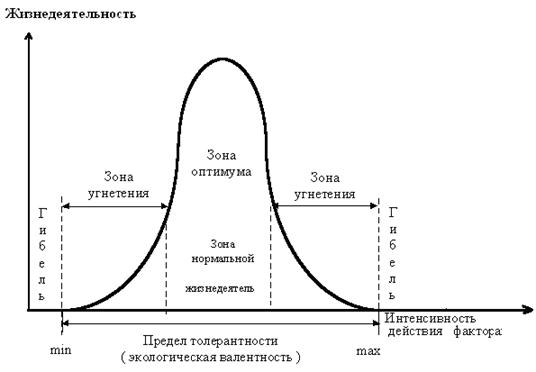
\includegraphics{img/tolerant.jpg}
    \caption{Кривая толерантноcти}
\end{figure}

\textbf{Анабиоз} -- обезвоживание клеток, пережидание в совершенно
неблагоприятных условиях существования

\textbf{Криптобиоз} -- замедление жизнедеятельности организма
(впадение в спячку, зимнее стояние лиственных деревьях)

\section{Закономерности действия факторов на организм}

\subsection{Закон оптиума}

Для каждого фактора существует область таких значений, при которых
жизнеспособность организма максимальна

\subsection{Закон Либиха}

Тот из факторов, который больше всего отклоняется от оптимума в сторону
минимума в данный момент ограничивает жизнедеятельность организма

\subsection{Закон Шелфорда}

Ограничивающим фактором может быть как минимум так и максимум
экологического воздействия

\subsubsection{Бочка Либиха}

\begin{figure}[H]
    \centering
    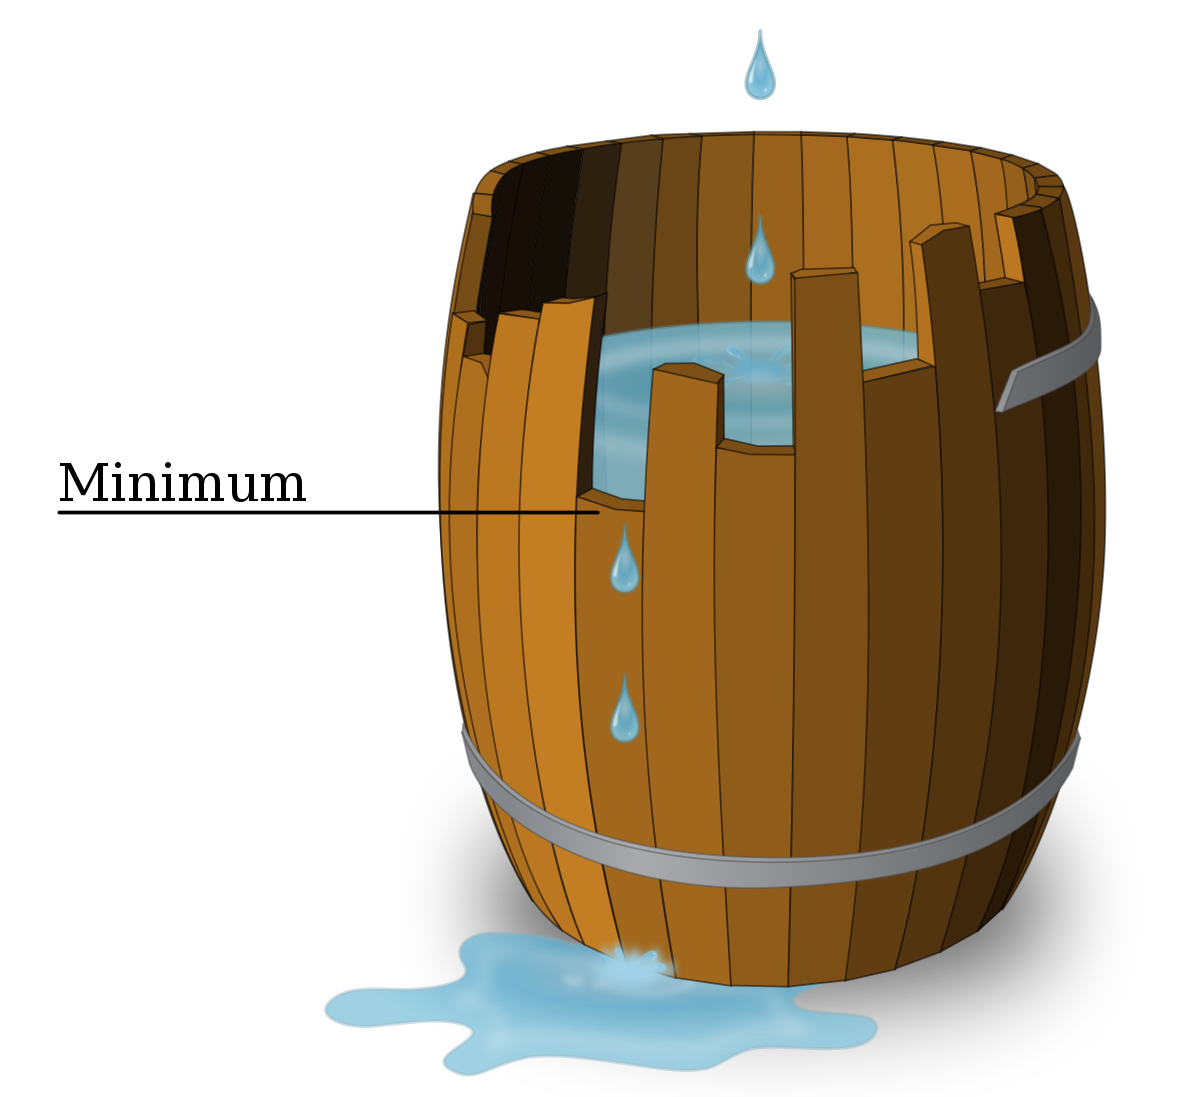
\includegraphics[scale=0.15]{img/libih.png}
    \caption{Бочка Либиха}
\end{figure}

Какими бы не были длинными доски, все равно вода выливается по
уровню минимальной доски

\subsection{Правило экологической индивидуальности}

В природе не существует двух видов с полным совпадением оптимумов
и критических точек по отношению к комплексу факторов

\section{Факторы}

Результат влияния какого-либо экологического фактора на организм
зависит не только от его количественного выражения, но и от того,
какой комбинацией и с какой интенсивность действуют другие факторы.

\subsection{4 вида взаимодействия факторов}

\begin{enumerate}
    \item \textbf{Аддитивность <<+>>} --
        просуммировать факторы
    \item \textbf{Антагонизм <<-->>} --
        наличие одного фактора ослабляет действие другого
    \item \textbf{Синергизм <<*>>} --
        усиление действия одного фактора при наличии другого
    \item \textbf{Нейтрализм <<0>>} --
        взаимодействие не выявлено
\end{enumerate}

\subsection{Абиотические факторы}

\begin{itemize}
    \item \textbf{Атмосферный воздух}
        \begin{enumerate}
            \item $N_2 \sim 78 \% (28 \frac{\text{г}}{\text{моль}})$
            \item $O_2 \sim 21 \% (32 \frac{\text{г}}{\text{моль}})$
            \item $\text{Инертные газы} \lesssim 1 \%$
            \item $CO_2 \sim 0.04 \% (44 \frac{\text{г}}{\text{моль}})$
        \end{enumerate}
        В реальном воздухе есть еще
        $H_2O (18 \frac{\text{г}}{\text{моль}})$

    \item \textbf{Электромагнитные излучения (солнечный свет)}

        \begin{figure}[H]
            \centering
            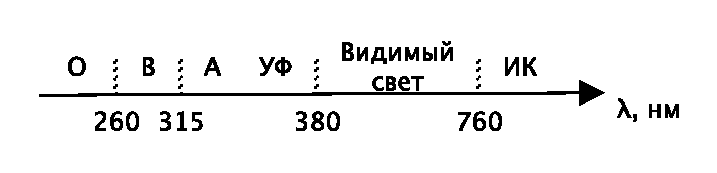
\includegraphics[scale=1]{img/light.pdf}
            \caption{Длины волн}
        \end{figure}

        Биологические процессы, связанные со светом
        \begin{itemize}
            \item Фотосинтез
            \item Выработка пигментов и витаминов
            \item Зрение, ориентация в пространстве
            \item Нагрев, передача тепла
            \item Фотопериодизм -- явление, связанное с реакцией
                организма на изменение продолжительности
                светлого времени суток
            \item Транспирация -- листья под действием
                солнечного света нагреваются, идет испарение воды
                с поверхности, вода падает на падает на почву и
                происходит питание организма
        \end{itemize}

        \begin{figure}[H]
            \centering
            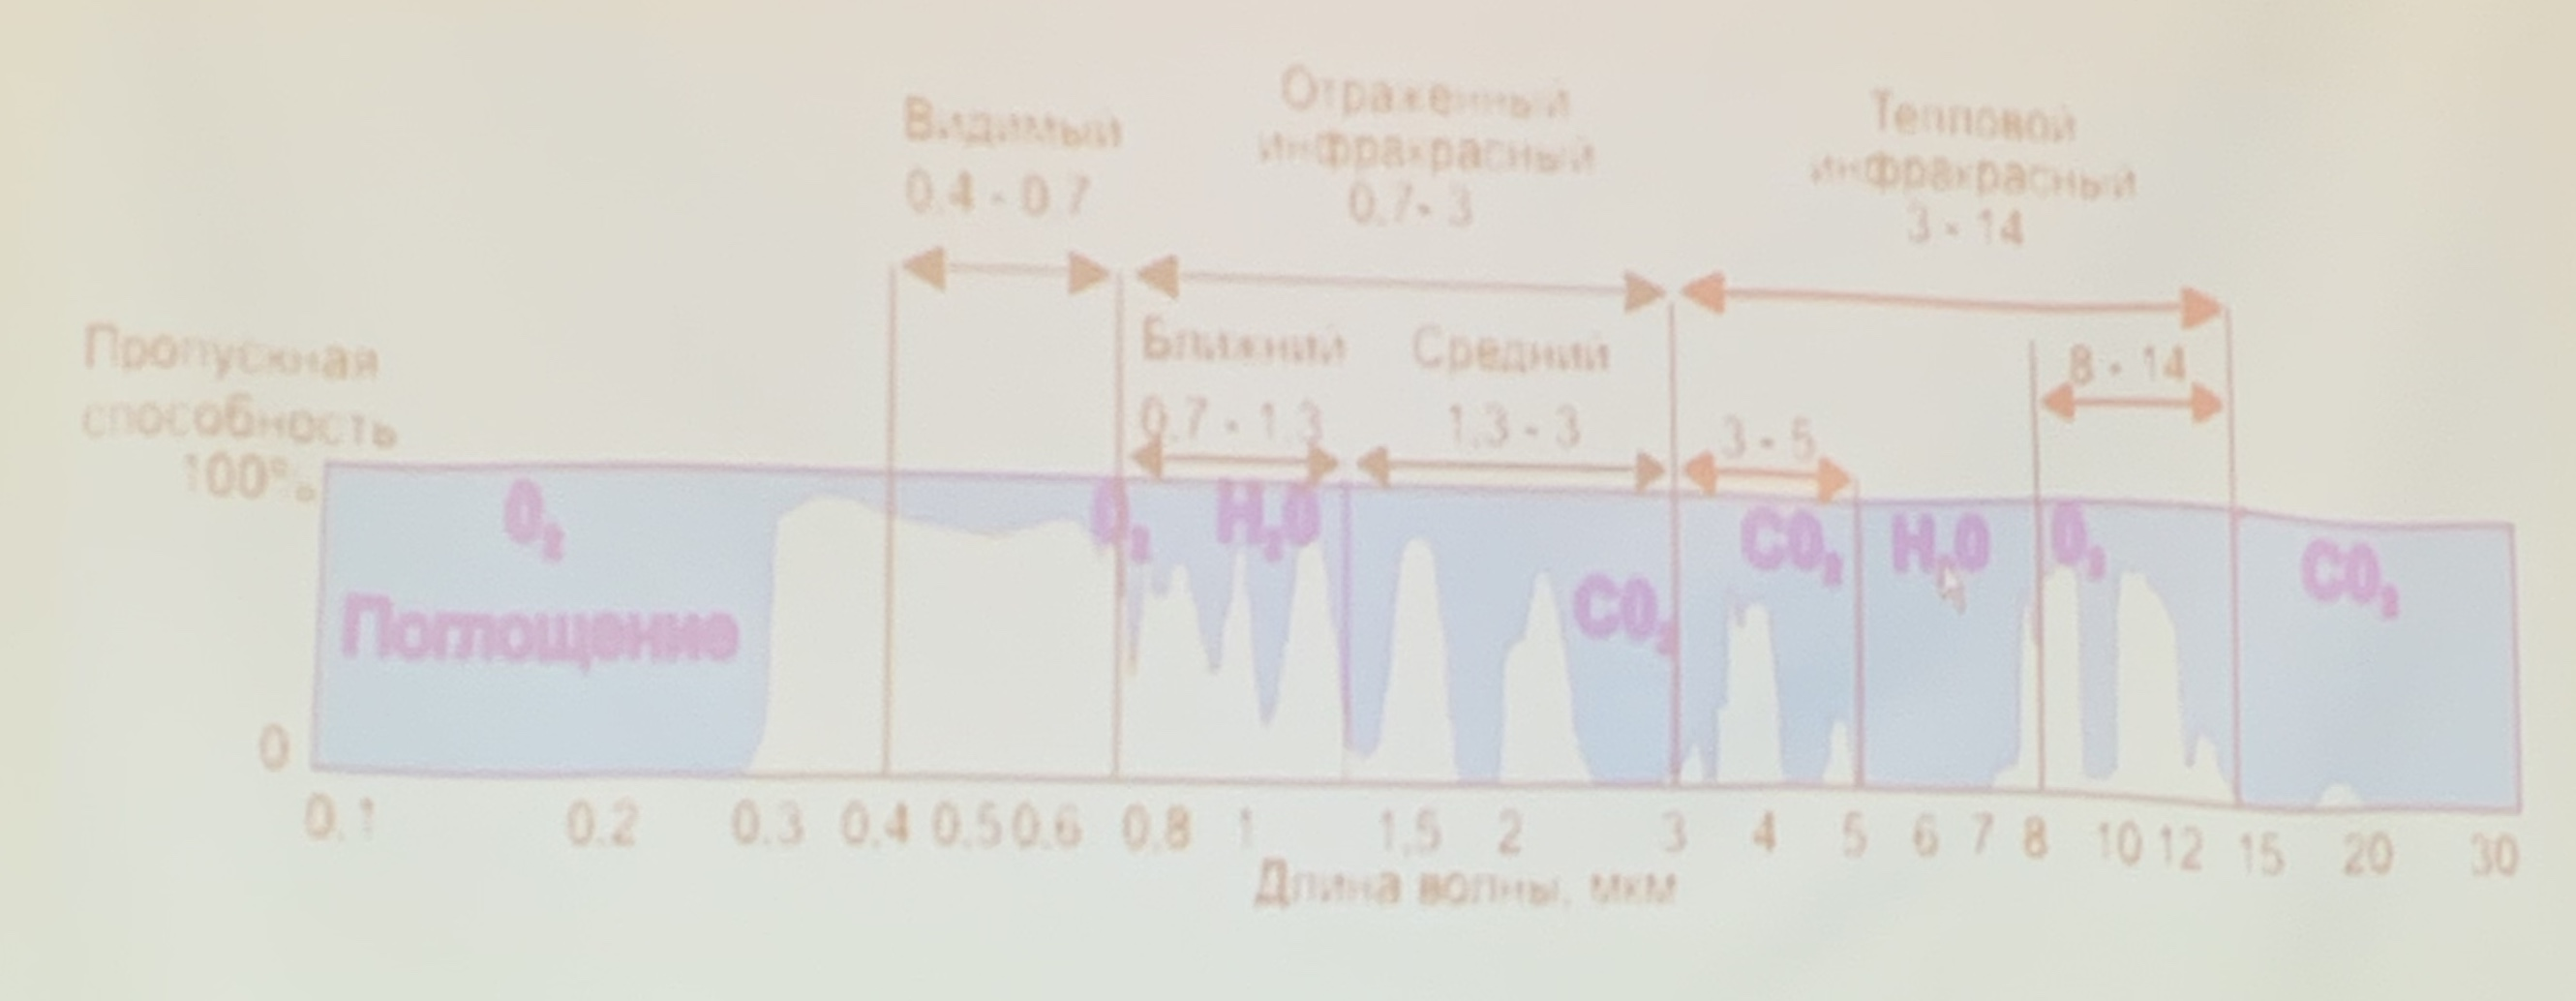
\includegraphics[scale=0.15]{img/cloud_effect.jpg}
            \caption{Парниковый эффект}
        \end{figure}

    \item \textbf{Вода}

        Свойства
        \begin{itemize}
            \item Проводит ток (дистиллированная вода -- диэлектрик)
            \item Высокая теплоемкость
                $4200 \frac{\text{Дж}}{\text{кг} \cdot \text{К}}$
            \item Может находиться в трех агрегатных состояниях
                (пар, вода, лёд)
            \item Является средой обитания для огромного количества
                живых организмов
        \end{itemize}

    \item \textbf{Температура}

        \begin{itemize}
            \item Точка кипения -- 100 градусов
            \item Точка замерзания -- 0 градусов
            \item Денатурация белков -- 40-50 градусов
        \end{itemize}

        Биогенные элементы
\end{itemize}

\subsection{Экологическая ниша}

\textbf{Экологическая ниша} -- это область таких значений экологических
факторов, при которых данный вид может существовать неограниченно долго

\subsubsection{3 состaвляющих экологической ниши}

\begin{enumerate}
    \item Трофическая (пищевая) ниша -- место в пищевой цепочке
    \item Пространственная ниша -- где обитает данный организм
    \item Временная ниша -- днем или ночью активен организм
\end{enumerate}

\subsection{Биотические факторы}

\begin{itemize}
    \item \textbf{Зоогенные} -- животные
        \begin{itemize}
            \item Гомотипические реации -- между особями одного вида
            \item Гетеротипические реакции -- между особями разного вида
        \end{itemize}
    \item \textbf{Фитогенный} -- растения
    \item \textbf{Микроорганизмы}
\end{itemize}

\section{Гомотипы}

\begin{itemize}
    \item Конкуренция внутривидовая

        \begin{itemize}
            \item Территория
            \item Противоположный пол
        \end{itemize}

    \item Групповой эффект --
        положительный эффект (проще выживать, охотиться)
    \item Массовый эффект
        -- особей уже слишком много, отрицательный эффект
\end{itemize}

\section{Принцип Оми}

Для каждой популяции существует оптимальная численность и
оптимальная плотность. Как недонаселенность, так и перенаселенность
негативно сказывается на популяции.

\section{Фитоген}

\begin{itemize}
    \item Прямые контактные взаимоотношения
        \begin{itemize}
            \item Механический
                (сплетение корней)
            \item Физиологический
                (симбиоз)

                Растения хищники, которые будут кого-то есть
        \end{itemize}

    \item Косвенные контактные взаимоотношения

        Изменение среды обитания, включая изменение светового режима.
        \textbf{Растения Эдификаторы} -- растения, которые относительно
        сильно изменяют среду обитания
\end{itemize}

\section{Среда обитания}

Среда обитания -- это часть природной среды, которая окружает живые
организмы и оказывает прямое или косвенное воздействие
на их состояния, развития, выживание и размножение.

\begin{table}[H]
    \centering
    \begin{tabular}{|l|l|l|l|l|}
        \hline
        Фактор & Водная & Наземно-  & Организменная & Почвенная \\
               &        & воздушная &               & \\
        \hline
        $t$ & Медленно & большая   & const & Средне \\
            & меняется & амплитуда &       & меняется \\
        \hline
        Свет $h \nu$ & Изначально     & Избыток & Темно & Почти \\
                     & мало, падает с &         &       & отсутствует \\
                     & увеличением    &         &       & \\
                     & глубины        &         &       & \\
        \hline
        $O_2$ & Расстворен    & Избыток & Недостаток & Недостаток \\
              & в среде,      &         &            &            \\
              & потенциальный &         &            &            \\
              & недостаток    &         &            &            \\
        \hline
        $H_2O$ & Избыток & Потенциальный & Достаточно & Недостаток \\
               &         & недостаток    &            &            \\
        \hline
        Плотность $\rho$ & $1000 \frac{\text{кг}}{\text{м}^3}$ &
                  $\frac{29}{22.4} = 1.3 \frac{\text{г}}{\text{л}} = 1.3 \frac{\text{кг}}{\text{м}^3}$
                         & & \\
        \hline
        Давление & $p = \rho g h + 1$ атм $=$ & 101325 Па & & \\
                 & $= 1000 \cdot 10 \cdot 10 = 10^5$ & & & \\
        \hline
    \end{tabular}
\end{table}

\subsection{Организменная среда обитания}

\begin{itemize}
    \item Эндопаразиты -- снаружи
    \item Эктопаразиты -- внутри
\end{itemize}
